\section{Introduction}

Quadrotor drones are  currently a hot topic in today’s society and has many promising uses now and in the future. Quadcopters are used as research platforms because of their simple design. They are for example used by the military, law enforcements, hobbyists and in commercial applications. Today the operational time for a quadcopter is generally far below what is desired. There is a high desire to increase the battery life of the quadcopters, at the very least not decrease it. Most multicopters have two pairs of fixed pitched propellers, one pair that goes clockwise and one pair that goes counter-clockwise (see figure \ref{dir}). Traditional quadcopters are controlled by changing the speed of the individual propellers. That way, it generates more or less thrust when required. This traditional method is not fast enough, and causes the multicopters to struggle in turbulent weather and wind conditions. Another main focus with quadcopters is the operational time. \\
\\
On this basis the Norwegian Defence Research Establishment has requested that we should do research on variable pitch. This makes the quadcopter mechanically more complex and heavy, but gives higher performance and the possibility of even flying inverted. This method can solve the current stability problem, and probably improve battery life if the quadcopter is running at constant RPM. Our project consists of researching the advantages and disadvantages of variable pitch. \\
\\
The project consists of building two quadcopters, one with variable pitch and one without. Both of them has to be less than 2.5 kilos (because of laws and regulations) and should be as similar as possible. We need to make a flight controller and create a method for the quadcopter so it can fly with an autopilot or radio controller. This have to be done for both of the quadcopters. These two quadcopters will then be tested to find out the pros and cons of variable pitch quadcopter flight. It’s important that we especially test the battery time and the response time, to find out the effect variable pitch has on these.\\
\\
This project will mostly be a research project and not a product development project. We are standing quite freely when choosing the design, hardware components and software implementation. Our main goal is the test data.
\\\\
\begin{figure}[h]
          \centering
            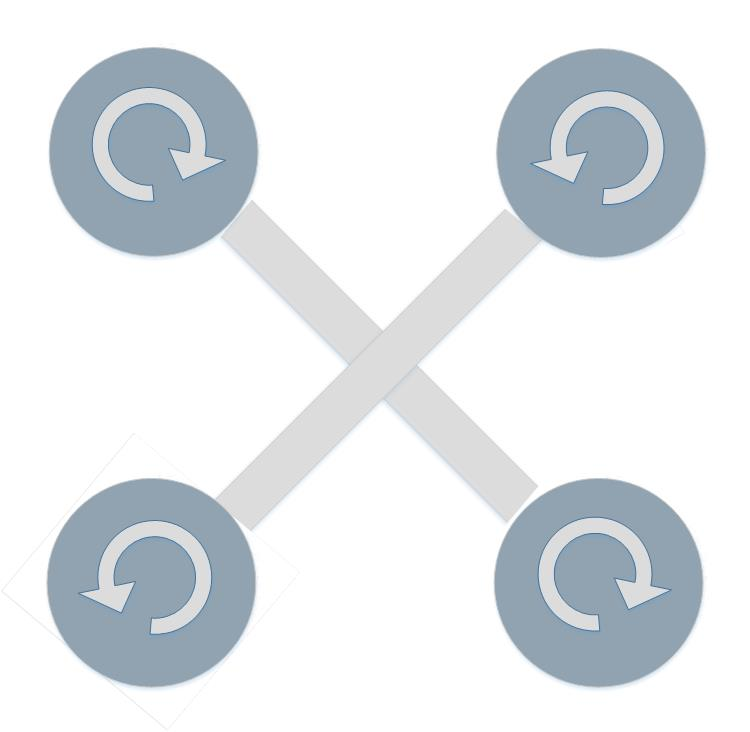
\includegraphics[scale = 0.33]{VAPIQ-PICTURES/dir_x_copter.jpg}
                \caption{Propeller direction}
            \label{dir}
\end{figure}